\section{Základné pojmy}
Pred samotným uvedením do problému, ktorým sa zaoberá táto práca je dôležité vysvetliť a definovať základné pojmy, ktoré sú spojené s danou problematikou a využívané v texte. 

\subsection{Heslo}
Heslo je prostriedok, pomocou ktorého je overená totožnosť používateľa. \cite{1} Pomocou neho vieme získať prístup k informáciam, dátam atď. ktoré sú pod ním uzamknuté. Teda iba ten, kto heslo pozná, môže pristupovať k týmto materiálom. Z tohto môžeme usúdiť, že heslo by malo byť dostatočne silné. Musí byť ťažko uhádnuteľné a komplexné. Jeho vlastník by ho mal ukryť pred odhalením alebo uhádnutím útočníka. Týmto nám vznikajú rôzne otázky: \textit{Aké miesto je bezpečné na ukrytie hesla? Kedy môžeme prehlásiť, že heslo je ,,silné''?}

\subsection{Autentizácia}
Proces, pri ktorej je overená totožnosť osoby, sa nazýva autentizácia. Predchádza ju proces identifikácie, kedy sa osoba ,,predstaví'' a povie, kto je. Systém ho ďalej v procese autentizácie ,,vyzve'', aby dokázal, že dotyčná osoba je naozaj tou, za ktorú sa prehlásil. Tým dôkazom myslíme vyššie spomínané heslo. \cite{2}
\par V praktickej rovine sú spôsoby autentizácie rôzne, ako napríklad: biometrický odtlačok, fráza vo forme hlasu, textového reťazca, číselný PIN a podobne \cite{3}. 

\subsection{Sila hesla} 
Uvažujme heslo ako textový reťazec. Sila hesla označuje stupeň obtiažnosti s akou ho neautorizovaná osoba dokáže uhádnuť \cite{4}. Heslo môže byť silné alebo slabé, v závislosti od toho, ako ťažké ho je uhádnuť \cite{4}. Slabé heslo je napríklad používanie iba malých písmen alebo iba číslic. Dôvod, prečo to tak je, je príliš malý priestor výberu znaku. Pri číselnom hesle hovoríme o priestore desiatich znakov. Uvažujme štandardnú telegrafnú abecedu s 26 písmenami. Potom je priestor pri použití hesla iba z malých písmen veľký 26 znakov. Útočník môže predpokladať, že používateľ má heslo zložené iba z číslic alebo iba z malých písmen\footnote{Možnosť použitia hesla iba z veľkých písmen nespomíname, pretože z matematického hľadiska náročnosti prelomenia hesla ide o rovnaký prípad ako pri malých písmenách.}. \par Preto na druhej strane hovoríme, že silné heslo je také heslo, ktoré obsahuje kombináciu veľkých a malých písmen a číslic. Už len kombináciou veľkých a malých písmen sa nám priestor zdvojnásobí. Abeceda veľkých písmen aj malých písmen má 26 znakov, čo je spolu 52 znakov. Zrazu je pre útočníka pri každom písmene nutné uvažovať, či sa použilo ako veľké, alebo ako malé. Z matematického hľadiska, teda z hľadiska permutácií sa celkový počet možných usporiadaní exponenciálne zvýši. Permutácia znamená usporiadanie.  


\begin{table}[ht]
\caption{Zložitosť prelomenia hesiel pomocou útoku brute-force podľa webovej stránky grc.com/haystack.htm}
\label{table:1}
\begin{tabular}{llll}
\textbf{Typ Hesla}        & \textbf{Heslo} & \textbf{Priestor} & \textbf{Počet možností} \\
Číslice (ďalej len C)     & 01234          & 10                & $1,11*10^5$             \\
Malé písmená (ďalej MP)   & heslo          & 26                & $1,24*10^7$             \\
MP + veľké písmená (VP)   & hEsLo          & 52                & $3,88*10^8$             \\
MP + VP + C               & h3sL0          & 62                & $9,31*10^8$             \\
MP + VP + C				  & h3sL0jeSiLn3   & 62				   & $3,28*10^{21}$			 \\
MP + VP + C + špec. znaky & h3sL0=\%SiLn3  & 95                & $5,46*10^{23}$           
\end{tabular}
\end{table}

\begin{table}[ht]
\begin{tabular}{lll}
\textbf{Heslo} & \textbf{\begin{tabular}[c]{@{}l@{}}Čas (online útok)\\ pri 1000 pokusoch/s\end{tabular}} &
  \textbf{\begin{tabular}[c]{@{}l@{}}Čas (offline útok)\\ pri miliarde pokusoch/s\end{tabular}} \\
01234 &				1,85 min            & 0,00000111 s \\
heslo &				3,43 hod            & 0,000124 s   \\
hEsLo &				4,49 dní            & 0,00388 s    \\
h3sL0 &				1,54 týždňov        & 0,00931 s    \\
h3sl0jeSiLn3 &		104 miliárd rokov	& 1043 rokov   \\
h3sLo=\%SiLn3 &		17,4 biliónov rokov & 1740 rokov   \\
\end{tabular}
\end{table}

\par Z tabuľky sme pozorovaním zistili, že rovnako ako bohatý priestor znakov je dôležitá aj dĺžka hesla. S použitím veľkých aj malých písmen pri dĺžke hesla 5 by bol útočník schopný zistiť naše heslo za veľmi krátky čas. Môžeme si z časových výsledkov všimnúť, že z praktického hľadiska skoro ani nezáleží, či použijeme C, MP, MP + VP alebo MP + VP + C, pokiaľ je heslo krátke. Najmä pri offline útoku zjavne vidieť, že vo všetkých prípadoch by stroj uhádol heslo doslova do sekundy.
\par Silu exponenciálneho rastu si všímame pri zmene dĺžky hesla na 12 znakov. Celá situácia sa dramaticky zmenila a kombinácie C, MP a VP už dávajú zmysel. Ďalší veľký skok spôsobilo pridanie špeciálnych znakov. Keďže zväčšili priestor rôznych znakov o viac ako polovicu, významná zmena je vidieť aj vo výsledkoch.
\par Predpokladajme, že útočník má informáciu, že používateľ vlastní heslo zložené iba z MP. Potom platí, že ak by používateľ zväčšil dĺžku hesla o jeden znak, útočník musí vykonať v priemere o 26 viac pokusov pri každej permutácii. \cite{5} 
\par Ďalej predpokladajme, že používateľ vlastní heslo zložené z MP, VP a C. Takáto kombinácia je dnes pri registrácii vo veľkej miere povinnosťou na rôznych webových stránkach. Potom platí, že pri zväčšení dĺžky hesla o jeden znak by sa zložitosť hesla nezvýšila iba 26, ale až 62-násobne. Z toho vyplýva, že útočník by musel mať 62-násobne väčší výkon, aby mohol za rovnaký čas zlomiť heslo z pôvodnou dĺžkou. Ten sa zvyšuje každé dva roky dvojnásobne, podľa Moorovho zákona. \cite{5} 
\newline \newline Táto úvaha spolu s ďalšími typmi útokov a ochranou pred nimi je hlbšie obsiahnutá v práci \cite{5}.

\subsection{Password manager}
Password manager (alebo po sl. správca hesiel) je aplikácia, ktorá umožňuje vytváranie, uchovávanie a používanie rôznych hesiel \cite{6}. Zhromažďuje ich na jednom mieste a vytvára pre používateľa prehľad jeho prístupových údajov. Tento ,,trezor'' je chránený master heslom.
\par Master heslo (často sa s ním stretnete v angl. forme ,,master password'') je heslo, ktoré je použité na sprístupnenie iných hesiel \cite{7}. Táto skutočnosť nám odhalila jednu pozitívnu a jednu negatívnu stranu password managerov všeobecne. Pozítivom je, že namiesto \textit{n} hesiel si stačí pamätať práve jedno heslo - master heslo. Týmto bolo rovno zodpovedané aj negatívum. Ak sa vieme jedným heslom dostať ku všetkým ostatným, stačí zlomiť master heslo a útočník získa všetky údaje v trezore, teda v password manageri.

\subsection{Šifrovanie}
\noindent Nasledujúci text vychádza zo zdroja \cite{8}. 
\par Šiforvanie je prepis otvoreného (čitateľného) textu do zašifrovaného textu, ktorý nazývame šifra. Abeceda, z ktorého vychádza otvorený text budeme označovať ako $\mathcal{P}$ a abecedu, z ktorého bude vychádzať zašifrovaný text budeme označovať ako $\mathcal{C}$.
\begin{equation}
e_k = \mathcal{P} \rightarrow \mathcal{C}
\end{equation}
\par Vidíme, že ide o zobrazenie. Toto zobrazenie je bijektívne, no nie vždy je tomu tak (napríklad pri znáhodnených šifrách). Je závislé na tajnom parametri $k$, ktorý nazývame kľúč. Ten patrí do množiny kľúčov $K$. V dnešných, moderných šifrách skoro vždy platí, že $\mathcal{P} \neq \mathcal{C}$, avšak v klasických šifrách bol opak úplne bežným úkazom (transpozičné, substitučné, homofónne šifry a podobne).
\par Aby vedel príjemca šifru prečítať, musí byť spomínané zobrazenie invertovateľné. To znamená, že musí byť použité inverzné zobrazenie 
\begin{equation}
d_k = \mathcal{C} \rightarrow \mathcal{P}
\end{equation}
také, aby platilo: $d_k(e_k(x)) = x$, kde $x$ je nezašifrovaná správa. Z týchto vzťahov je zrejmé, že príjemca musí použiť totožný kľúč $k$ s kľúčom odosielateľa, aby sa dostal k $x$. Útočník sa snaží nájsť tento kľúč. Preto čím väčšia je množina $K$, tým náročnejšie, niekedy až nemožné z hľadiska výpočtovej sily, je nájsť $k$.
\par V dobe klasických šifier (obdobie do roku 1945) väčšinou spočívala bezpečnosť niektorých algoritmov v ukrytí algoritmu samotného. To ale nie je správny prístup, pretože podľa Kerckhoffovho princípu \cite{9} má bezpečnosť šifrovacieho algoritmu spočívať na utajení kľúča, nie algoritmu samotného. Týmto princípom sa riadia dnešné, moderné šifry dodnes. 

\section{Problém password managerov}
Password manager ponúka používateľovi mnohé výhody a možnosti. Od generátora hesiel a ich automatického vyplnenia pri prihlasovaní do stránok, cez synchronizáciu medzi zariadeniami, zálohovanie, až po automatickú, pravidelnú zmenu jednotlivých hesiel. Napriek tomu existuje problém týchto managerov, ktorý ostal neriešený. Jemu sa bude táto kapitola venovať.

\subsection{Súčasný stav na trhu}
Ak hovoríme o heslách, priame (explicitné) používanie nižšie uvedených aplikácií pri dennom používaní je minimálne. A to vďaka automatickému vypĺňaniu hesla. Používateľ vstúpi na webovú stránku alebo do aplikácie. Pred vstupom sa musí prihlásiť do svojho účtu. Tam mu password manager výzvou ponúkne automatické vyplnenie (angl. výraz ,,autofill'') prihlasovacieho mena a hesla. Toto poskytuje vysokú úroveň komfortu. Používateľ nielen že nemusí vypisovať svoje prihlasovacie údaje manuálne, ale aj ich bezpečnosť porástla na vyššiu úroveň. Vďaka password manageru.
\par Podobne to funguje pri registrácii nového konta. Niektoré password manager aplikácie ponúknu náhodne vygenerované silné heslo (iCloud Keychain, \cite{10}). Používateľ sa môže rozhodnúť ho prijať. V takom prípade sa heslo pre vytvorený účet uloží do password manageru a ten ho pri každom ďalšom prihlásení vyplní. 
\subsubsection{LastPass} 
LastPass patrí medzi jeden z najpopulárnejších, čo sa týka počtu používateľov \cite{11}. Všetky heslá a ostatný obsah sú uzamknuté pod jedným master heslom. LastPass ale povoľuje aj vstup do jeho aplikácie pomocou biometrickej autentifikácie, ktorú väčšina smartfónov podporuje. Používateľ tak nemusí každý raz písať dlhé master heslo. Jediné, čo stačí, je priložiť prst, či pozrieť sa na smartfón (sken tváre). 
\par LastPass je client-server aplikácia. To znamená, že niektoré operácie a procesy prebiehajú na strane kienta, teda priamo v danom zariadení, ktoré používateľ drží a niektoré prebiehajú na strane LastPass serverov. Samotné šifrovanie, aj dešifrovanie prebieha na strane zariadenia \cite{12}. LastPass vytvorí kľúč z master hesla pomocou šifry AES (Advanced Encryption Standard) s hašovaním PBKDF2 (Key Derivation Function), SHA (Secure Hash Algorithm) s pridaným saltom \cite{13}. Týmto algoritmom sa bližšie venujeme v X.X (TODO číslo sekcie kde budem vysvetľovať AES princíp a hašovanie).
\par Dáta sú synchronizované pomocou serverov, čo umožňuje zálohovanie a synchronizáciu medzi zariadeniami. Dátový prenos po sieti je chránený pomocou TLS/SSL (\cite{14} sa bližšie venuje tomuto protokolu). LastPass v bezpečnosti pokračuje v možnosti dvojfaktorovej autorizácie a overovania na základe lokácie: kedykoľvek sa užívateľ prihlasuje do aplikácie z inej lokality, je vyzvaný prostredníctvom emailu s linkom, ktorý po otvorení overí používateľa ako verifikovaného. LastPass má mnoho možností, ako napríklad zdieľanie hesiel s iným LastPass účtom, generovanie hesiel s používateľom zvolenou dĺžkou a podmienkami, hodnotenie sily hesiel (systém usúdi, či je heslo dostatočne bezpečné), či import hesiel pomocou CSV súboru alebo iného password manageru.
\newline
\begin{figure}[ht]
  \centering
  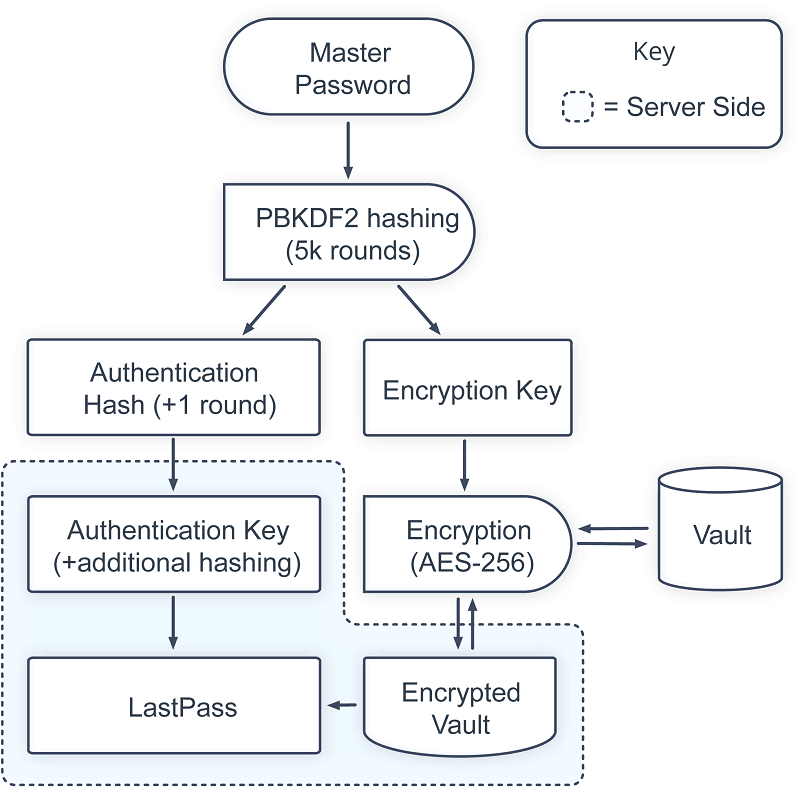
\includegraphics[width=8cm]{img/lastpass.png}
  \caption{Schéma šifrovania aplikácie LastPass.}
\end{figure}

\subsubsection{Dashlane}
Tento password manager je tiež vysoko využívaný \cite{15}. Jedna z jeho jedinečných funkcionalít je automatická zmena hesla \cite{16}. Používateľ si môže vybrať v zozname svojich hesiel, ktoré by sa mali automaticky meniť. Dashlane tak bude pravidelne generovať nové, komplexné heslá pre vybrané položky. Keďže medzi rôznymi webovými stránkami nie je jednotná architektúra a dizajn, nie všetky položky účtov vie Dashlane meniť automaticky. V takom prípade si užívateľ vie meniť heslo pre danú položku iba manuálne, v konkrétnej aplikácii alebo webovej stránke pre službu, ku ktorej prislúcha daný účet v Dashlane.
\par Tak ako LastPass, aj tento password manager dominuje silnou bezpečnosťou. Podporuje dvojfaktorovú autentifikáciu (dodatočné overenie po prvotnom prihlásení, viac v \cite{17}), šifru AES a synchronizáciu medzi zariadeniami. Mnohé z funkcionalít a možností má spoločné s aplikáciou LastPass. Nebudeme ich opäť spomínať, nakoľko cieľom tejto kapitoly je iba ukázať už existujúce vymoženosti rôznych password managerov.

\subsubsection{iCloud Keychain}
\par Za spomenutie určite stojí vstavaný password manager od spoločnosti Apple. Obsahuje určité funkcionality password managera, ktoré sú základnou súčasťou každého iOS, iPadOS, či MacOS zariadenia. Každý používateľ nejakého Apple zariadenia je identifikovaný pomocou AppleID konta. K nemu má pridelené cloud úložisko, kde sa mu všetky dáta zálohujú a synchronizujú so všetkými Apple zariadeniami.
\par Okrem fotiek, poznámok, kontaktov atď tam sú uložené aj heslá z Keychainu. Keychain si pamätá nielen heslá, ale aj certifikáty, dôležité pri rôznych verifikáciach vrámci systému. Taktiež si pamätá kľúče. Sú verejné, ale aj súkromné, systém ich používa napríklad pri používaní iMessage aplikácie na posielanie správ. Sú šifrované pomocou šifry RSA a dĺžka kľúča je niekedy až 2048 bitov. \\

\par Z ostatných managerov ukážeme zopár ďalších funkcionalít, ktoré neboli spomenuté, respektíve ich LastPass, Dashlane, či Keychain neposkytujú.
\par 1Password ponúka takzvaný ,,Emergancy kit''. Po vytvorení 1Password účtu je používateľovi poskytnutý dokument. Následne je vyzvaný, aby si ho vytlačil, prípadne uložil na pamäťové médium. Dokument obsahuje prihlasovacie údaje a master heslo. Taktiež obsahuje QR kód, ktorý automaticky vyplní tieto dáta pri núdzovom prihlasovaní. \\

\begin{figure}[ht]
  \centering
  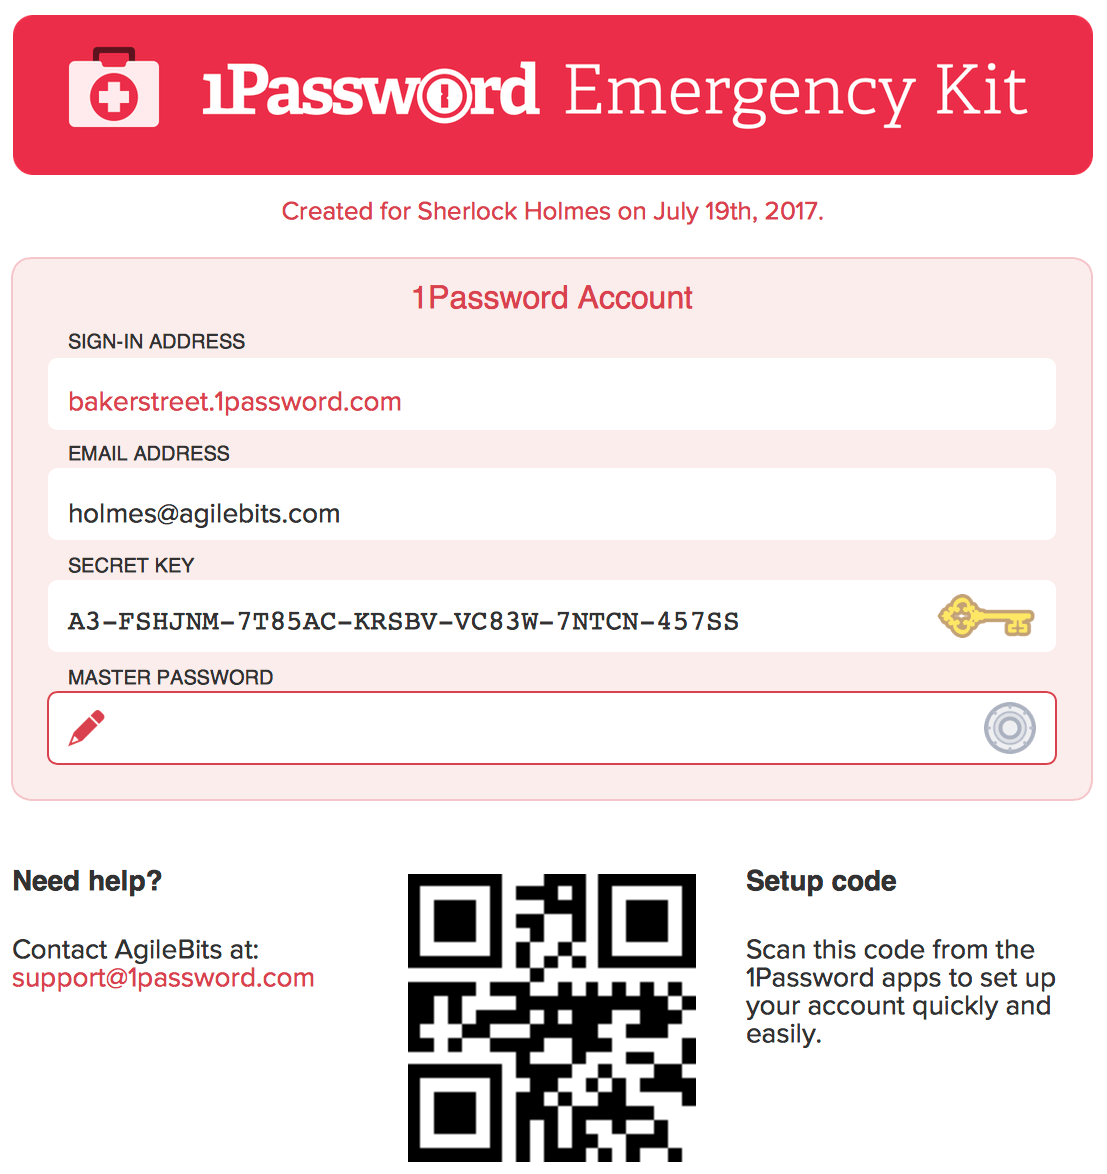
\includegraphics[width=8cm]{img/1pass.png}
  \caption{Emergency kit od 1Password - ukážka pdf súboru, ktorý používateľ obdrží.}
\end{figure}

\par Password manager Remembear ponúka jednoduchú aktiváciu aplikácie na novom zariadení prostredníctvom QR kódu. Za spomenutie stojí aj menej známy správca, konkrétne Myki. \par Myki ako jeden z mála nepoužíva svoje servery na zálohovanie a ukladanie hesiel. Namiesto toho využíva server iba ako sprostredkovateľa \cite{18} spojenia keď nastáva synchronizácia medzi zariadeniami. Teda, používať Myki na viacerých zariadeniach je akousi formou ,,zálohy''.
\par Vyššie spomenuté aplikácie fungujú na rôznych platformách: verzia pre smartfóny (iOS, Android), počítače (Windows, MacOS, Linux), inteligentné hodinky a podobne.

\subsection{Nízka popularita}
Sem pôjde analýza prieskumov ako ľudia používajú password managere všeobecne (mizerné výsledky vzhľadom na popularitu).

\section{Recitácia}
Citujem všetky zdroje v \textbf{bibliography.bib}, \cite{t00, t01, t02, t03, kniha, kniha2, kniha3, small, big, cs, koll, kap, tug, knuth, zbornik, prispevok}. \newline Good luck.
\section{Možnosti anonymizácie}
\noindent Anonymizácia znamená zmena alebo úprava údajov tak, aby sa podľa nich nedala jednoznačne určiť osoba, ktorej tieto údaje patria \cite{t01}. Existuje niekoľko spôsobov, ktorými môžeme dosiahnuť rôznu úroveň anonymizácie na internete: od mazania cookies súborov po ukončení prehliadania webových stránok až po používanie operačných systémov, ktoré sú na anonymite založené; od bezplatných možností až po komerčné verzie.  
\newline Nasleduje priblíženie niektorých možnosti anonymizácie.

\subsection{Súkromné prehliadanie}
\noindent Najpoužívanejšie internetové prehliadače súčasnosti majú v sebe zabudovanú funkcionalitu, ktorá dokáže čiastočne anonymizovať prístup na internet. Táto funkcionalita blokuje ukladanie navštívených stránok do histórie a nezaznamenáva súbory, ktoré sa stiahnu z~internetu. \acrshort{sw} a \acrlong{hw} sú skratky.

\begin{table}[!htbp]
\caption{Moduly a ich funkcie pri anonymizácii}
\label{modulyVlastnosti}
\begin{center}
\begin{tabular}{p{4cm}|c|c|c|c|c|c|c|c|c|c|c|c|c|c|c}
& \multicolumn{14}{c}%
	 {\textbf{Funkcia}}\\ \hline
&&&& & &\multicolumn{8}{c}%
	 {Modifikácia}\\ 
\textbf{Modul} &\begin{sideways} zobrazenie hlavičky \end{sideways} &\begin{sideways} blokovanie skriptov \end{sideways} &\begin{sideways} zmena IP \end{sideways} & \begin{sideways} zmena lokalizácie \end{sideways} & \begin{sideways} zmazanie/blokovanie cookies \end{sideways} & \begin{sideways} blokovanie trackerov \end{sideways}  & \begin{sideways} popis \end{sideways} & \begin{sideways}používateľský agent\end{sideways} & \begin{sideways} kódové označenie prehliadača \end{sideways} & \begin{sideways} názov prehliadača \end{sideways} & \begin{sideways} verzia prehliadača \end{sideways} & \begin{sideways} platforma \end{sideways} & \begin{sideways} výrobca prehliadača \end{sideways} & \begin{sideways} označenie výrobcu prehliadača \end{sideways} \\ \hline
User agent switcher & & & & & &  & X & X & X & X & X & X & X & X  \\ \hline
Ghostery &  && & & X & X &  &  & & & & & & \\  \hline
Better privacy && &  & & X &  &  &  & & & & & & \\  \hline
Anonymox &  && X & X & X &  & X & X & & & & & & \\  \hline
Modify headers & & &  &  & X &  &  & X &  &  &  & & &  \\  \hline
Request policy & & &  &  & & X  &  &  &  &  &  & & &   \\  \hline
Live HTTP headers & X& &  &  & &  &  &  &  &  &  & & &   \\  \hline
User agent awitcher for chrome & & &  &  & &  & X & X &  &  &  & & &   \\  \hline
Header hacker & & &  &  & &  & X & X & X & X & X & X & X & X    \\  \hline
Mod header & & &  &  & &  & X & X & X & X & X & X & X & X    \\  \hline
Script no & &X &  &  & &  &  &  &  &  &  &  &  &     \\  \hline
No script & &X &  &  & &  &  &  &  &  &  &  &  &     \\  \hline
Proxify it & & &X  & X & &  &  &  &  &  &  &  &  &     \\  \hline
I'm not here & & &  & X & &  &  &  &  &  &  &  &  &     \\  \hline
Get anonymous personal edition & &X &X &X &X&X &  &  &  &  &  &  &  &     \\  \hline
Anonymous browsing toolbar & & & X & X & &  &  &  &  &  &  &  &  &     \\  \hline
Easy hide your IP and surf anonymously & & & X & X& &  &  & X & X & X & X &  &  &     \\  \hline
\end{tabular}
\end{center}
\end{table}

\subsection{Anonymná sieť}
\noindent Anonymná sieť je sieť serverov, medzi ktorými dáta prechádzajú šifrované. V anonymných sieťach dáta prechádzajú z počítača používateľa, odkiaľ bola požiadavka poslaná, cez viaceré proxy smerovače, z ktorých každý správu doplní o smerovanie a zašifruje vlastným kľúčom. Cesta od ...


\subsection{Funkcionalita}
\noindent  Rozšírenie tiež okrem splnenia špecifikácie malo pre prehľadnosť a overenie funkčnosti zobrazovať údaje, ktoré boli na server odoslané. Zoznam údajov odoslaných na server, sa mal ukladať do krátkodobej histórie, aby nemal používateľ k dispozícií len najnovšie údaje, ale aj údaje odoslané v nejakom časovom období. Nejaky listing z priloh \ref{lst:sublime}.

\subsubsection{Funkcionalita2}
\noindent Samozrejmosťou bolo nastavenie zapnutia rozšírenia pri štarte, prípadne interval zmeny odosielaných údajov.

\subsection{Vzhľad}
\noindent Dôležitou požiadavkou kladenou na rozšírenie bolo príjemné používateľské rozhranie. Z~tohto dôvodu malo rozšírenie obsahovať zoznam modifikovaných vlastností a tlačidlo pre prístup k nastaveniam rozšírenia v jednoduchej a praktickej forme. Predpokladaný vzhľad je zobrazený na obrázku č. \ref{vzhladobr}.
\begin{figure}[!htbp]
  \centering
  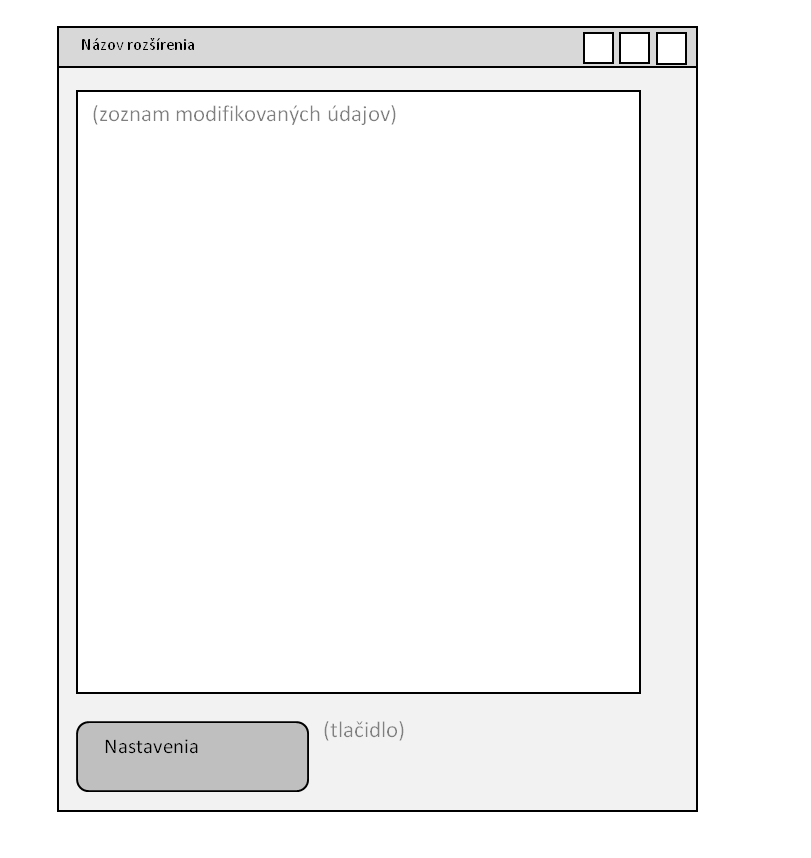
\includegraphics[width=8cm]{img/vzhlad.png}
  \caption{Predpokladaný vzhľad rozšírenia.}
  \label{vzhladobr}
\end{figure}	 
\noindent Dôležitou požiadavkou kladenou na rozšírenie bolo príjemné používateľské rozhranie.\cite{t00} Z~tohto dôvodu malo rozšírenie obsahovať zoznam modifikovaných vlastností a tlačidlo pre prístup k nastaveniam rozšírenia v jednoduchej a praktickej forme. Predpokladaný vzhľad je zobrazený na obrázku č. \ref{vzhladobr}.

\begin{algorithm}
\scriptsize
\begin{algorithmic}
 \STATE <text>
 \IF{<condition>} \STATE {<text>} \ELSE \STATE{<text>} \ENDIF
 \IF{<condition>} \STATE {<text>} \ELSIF{<condition>} \STATE{<text>} \ENDIF
 \FOR{<condition>} \STATE {<text>} \ENDFOR
 \FOR{<condition> \TO <condition> } \STATE {<text>} \ENDFOR
 \FORALL{<condition>} \STATE{<text>} \ENDFOR
 \WHILE{<condition>} \STATE{<text>} \ENDWHILE
 \REPEAT \STATE{<text>} \UNTIL{<condition>}
 \LOOP \STATE{<text>} \ENDLOOP
 \REQUIRE <text>
 \ENSURE <text>
 \RETURN <text>
 \PRINT <text>
 \COMMENT{<text>}
 \AND, \OR, \XOR, \NOT, \TO, \TRUE, \FALSE
\end{algorithmic}
\caption{Ukážka príkazov pre algorithmic}  
\label{alg:preview}  
\end{algorithm}

\begin{lstlisting}[
  caption={Ukážka algoritmu},
  label={lst:main-c},
  language=c
]
/* Hello World program */

#include<stdio.h>

struct cpu_info {
    long unsigned utime, ntime, stime, itime;
    long unsigned iowtime, irqtime, sirqtime;
};

main()
{
    printf("Hello World");
}
\end{lstlisting}